
%% bare_conf.tex
%% V1.4b
%% 2015/08/26
%% by Michael Shell
%% See:
%% http://www.michaelshell.org/
%% for current contact information.
%%
%% This is a skeleton file demonstrating the use of IEEEtran.cls
%% (requires IEEEtran.cls version 1.8b or later) with an IEEE
%% conference paper.
%%
%% Support sites:
%% http://www.michaelshell.org/tex/ieeetran/
%% http://www.ctan.org/pkg/ieeetran
%% and
%% http://www.ieee.org/

%%*************************************************************************
%% Legal Notice:
%% This code is offered as-is without any warranty either expressed or
%% implied; without even the implied warranty of MERCHANTABILITY or
%% FITNESS FOR A PARTICULAR PURPOSE! 
%% User assumes all risk.
%% In no event shall the IEEE or any contributor to this code be liable for
%% any damages or losses, including, but not limited to, incidental,
%% consequential, or any other damages, resulting from the use or misuse
%% of any information contained here.
%%
%% All comments are the opinions of their respective authors and are not
%% necessarily endorsed by the IEEE.
%%
%% This work is distributed under the LaTeX Project Public License (LPPL)
%% ( http://www.latex-project.org/ ) version 1.3, and may be freely used,
%% distributed and modified. A copy of the LPPL, version 1.3, is included
%% in the base LaTeX documentation of all distributions of LaTeX released
%% 2003/12/01 or later.
%% Retain all contribution notices and credits.
%% ** Modified files should be clearly indicated as such, including  **
%% ** renaming them and changing author support contact information. **
%%*************************************************************************


% *** Authors should verify (and, if needed, correct) their LaTeX system  ***
% *** with the testflow diagnostic prior to trusting their LaTeX platform ***
% *** with production work. The IEEE's font choices and paper sizes can   ***
% *** trigger bugs that do not appear when using other class files.       ***                          ***
% The testflow support page is at:
% http://www.michaelshell.org/tex/testflow/



\documentclass[conference]{IEEEtran}
% Some Computer Society conferences also require the compsoc mode option,
% but others use the standard conference format.
%
% If IEEEtran.cls has not been installed into the LaTeX system files,
% manually specify the path to it like:
% \documentclass[conference]{../sty/IEEEtran}
% Some very useful LaTeX packages include:
% (uncomment the ones you want to load)


% *** MISC UTILITY PACKAGES ***
%
%\usepackage{ifpdf}
% Heiko Oberdiek's ifpdf.sty is very useful if you need conditional
% compilation based on whether the output is pdf or dvi.
% usage:
% \ifpdf
%   % pdf code
% \else
%   % dvi code
% \fi
% The latest version of ifpdf.sty can be obtained from:
% http://www.ctan.org/pkg/ifpdf
% Also, note that IEEEtran.cls V1.7 and later provides a builtin
% \ifCLASSINFOpdf conditional that works the same way.
% When switching from latex to pdflatex and vice-versa, the compiler may
% have to be run twice to clear warning/error messages.






% *** CITATION PACKAGES ***
%
%\usepackage{cite}
% cite.sty was written by Donald Arseneau
% V1.6 and later of IEEEtran pre-defines the format of the cite.sty package
% \cite{} output to follow that of the IEEE. Loading the cite package will
% result in citation numbers being automatically sorted and properly
% "compressed/ranged". e.g., [1], [9], [2], [7], [5], [6] without using
% cite.sty will become [1], [2], [5]--[7], [9] using cite.sty. cite.sty's
% \cite will automatically add leading space, if needed. Use cite.sty's
% noadjust option (cite.sty V3.8 and later) if you want to turn this off
% such as if a citation ever needs to be enclosed in parenthesis.
% cite.sty is already installed on most LaTeX systems. Be sure and use
% version 5.0 (2009-03-20) and later if using hyperref.sty.
% The latest version can be obtained at:
% http://www.ctan.org/pkg/cite
% The documentation is contained in the cite.sty file itself.






% *** GRAPHICS RELATED PACKAGES ***
%
\ifCLASSINFOpdf
  % \usepackage[pdftex]{graphicx}
  % declare the path(s) where your graphic files are
  % \graphicspath{{../pdf/}{../jpeg/}}
  % and their extensions so you won't have to specify these with
  % every instance of \includegraphics
  % \DeclareGraphicsExtensions{.pdf,.jpeg,.png}
\else
  % or other class option (dvipsone, dvipdf, if not using dvips). graphicx
  % will default to the driver specified in the system graphics.cfg if no
  % driver is specified.
  % \usepackage[dvips]{graphicx}
  % declare the path(s) where your graphic files are
  % \graphicspath{{../eps/}}
  % and their extensions so you won't have to specify these with
  % every instance of \includegraphics
  % \DeclareGraphicsExtensions{.eps}
\fi
% graphicx was written by David Carlisle and Sebastian Rahtz. It is
% required if you want graphics, photos, etc. graphicx.sty is already
% installed on most LaTeX systems. The latest version and documentation
% can be obtained at: 
% http://www.ctan.org/pkg/graphicx
% Another good source of documentation is "Using Imported Graphics in
% LaTeX2e" by Keith Reckdahl which can be found at:
% http://www.ctan.org/pkg/epslatex
%
% latex, and pdflatex in dvi mode, support graphics in encapsulated
% postscript (.eps) format. pdflatex in pdf mode supports graphics
% in .pdf, .jpeg, .png and .mps (metapost) formats. Users should ensure
% that all non-photo figures use a vector format (.eps, .pdf, .mps) and
% not a bitmapped formats (.jpeg, .png). The IEEE frowns on bitmapped formats
% which can result in "jaggedy"/blurry rendering of lines and letters as
% well as large increases in file sizes.
%
% You can find documentation about the pdfTeX application at:
% http://www.tug.org/applications/pdftex





% *** MATH PACKAGES ***
%
%\usepackage{amsmath}
% A popular package from the American Mathematical Society that provides
% many useful and powerful commands for dealing with mathematics.
%
% Note that the amsmath package sets \interdisplaylinepenalty to 10000
% thus preventing page breaks from occurring within multiline equations. Use:
%\interdisplaylinepenalty=2500
% after loading amsmath to restore such page breaks as IEEEtran.cls normally
% does. amsmath.sty is already installed on most LaTeX systems. The latest
% version and documentation can be obtained at:
% http://www.ctan.org/pkg/amsmath





% *** SPECIALIZED LIST PACKAGES ***
%
%\usepackage{algorithmic}
% algorithmic.sty was written by Peter Williams and Rogerio Brito.
% This package provides an algorithmic environment fo describing algorithms.
% You can use the algorithmic environment in-text or within a figure
% environment to provide for a floating algorithm. Do NOT use the algorithm
% floating environment provided by algorithm.sty (by the same authors) or
% algorithm2e.sty (by Christophe Fiorio) as the IEEE does not use dedicated
% algorithm float types and packages that provide these will not provide
% correct IEEE style captions. The latest version and documentation of
% algorithmic.sty can be obtained at:
% http://www.ctan.org/pkg/algorithms
% Also of interest may be the (relatively newer and more customizable)
% algorithmicx.sty package by Szasz Janos:
% http://www.ctan.org/pkg/algorithmicx




% *** ALIGNMENT PACKAGES ***
%
%\usepackage{array}
% Frank Mittelbach's and David Carlisle's array.sty patches and improves
% the standard LaTeX2e array and tabular environments to provide better
% appearance and additional user controls. As the default LaTeX2e table
% generation code is lacking to the point of almost being broken with
% respect to the quality of the end results, all users are strongly
% advised to use an enhanced (at the very least that provided by array.sty)
% set of table tools. array.sty is already installed on most systems. The
% latest version and documentation can be obtained at:
% http://www.ctan.org/pkg/array                                     


% IEEEtran contains the IEEEeqnarray family of commands that can be used to
% generate multiline equations as well as matrices, tables, etc., of high
% quality.




% *** SUBFIGURE PACKAGES ***
%\ifCLASSOPTIONcompsoc
%  \usepackage[caption=false,font=normalsize,labelfont=sf,textfont=sf]{subfig}
%\else
%  \usepackage[caption=false,font=footnotesize]{subfig}
%\fi
% subfig.sty, written by Steven Douglas Cochran, is the modern replacement
% for subfigure.sty, the latter of which is no longer maintained and is
% incompatible with some LaTeX packages including fixltx2e. However,
% subfig.sty requires and automatically loads Axel Sommerfeldt's caption.sty
% which will override IEEEtran.cls' handling of captions and this will result
% in non-IEEE style figure/table captions. To prevent this problem, be sure
% and invoke subfig.sty's "caption=false" package option (available since
% subfig.sty version 1.3, 2005/06/28) as this is will preserve IEEEtran.cls
% handling of captions.
% Note that the Computer Society format requires a larger sans serif font
% than the serif footnote size font used in traditional IEEE formatting
% and thus the need to invoke different subfig.sty package options depending
% on whether compsoc mode has been enabled.
%
% The latest version and documentation of subfig.sty can be obtained at:
% http://www.ctan.org/pkg/subfig




% *** FLOAT PACKAGES ***
%
%\usepackage{fixltx2e}
% fixltx2e, the successor to the earlier fix2col.sty, was written by
% Frank Mittelbach and David Carlisle. This package corrects a few problems
% in the LaTeX2e kernel, the most notable of which is that in current
% LaTeX2e releases, the ordering of single and double column floats is not
% guaranteed to be preserved. Thus, an unpatched LaTeX2e can allow a
% single column figure to be placed prior to an earlier double column
% figure.
% Be aware that LaTeX2e kernels dated 2015 and later have fixltx2e.sty's
% corrections already built into the system in which case a warning will
% be issued if an attempt is made to load fixltx2e.sty as it is no longer
% needed.
% The latest version and documentation can be found at:
% http://www.ctan.org/pkg/fixltx2e


%\usepackage{stfloats}
% stfloats.sty was written by Sigitas Tolusis. This package gives LaTeX2e
% the ability to do double column floats at the bottom of the page as well
% as the top. (e.g., "\begin{figure*}[!b]" is not normally possible in
% LaTeX2e). It also provides a command:
%\fnbelowfloat
% to enable the placement of footnotes below bottom floats (the standard
% LaTeX2e kernel puts them above bottom floats). This is an invasive package
% which rewrites many portions of the LaTeX2e float routines. It may not work
% with other packages that modify the LaTeX2e float routines. The latest
% version and documentation can be obtained at:
% http://www.ctan.org/pkg/stfloats
% Do not use the stfloats baselinefloat ability as the IEEE does not allow
% \baselineskip to stretch. Authors submitting work to the IEEE should note
% that the IEEE rarely uses double column equations and that authors should try
% to avoid such use. Do not be tempted to use the cuted.sty or midfloat.sty
% packages (also by Sigitas Tolusis) as the IEEE does not format its papers in
% such ways.
% Do not attempt to use stfloats with fixltx2e as they are incompatible.
% Instead, use Morten Hogholm'a dblfloatfix which combines the features
% of both fixltx2e and stfloats:
%
% \usepackage{dblfloatfix}
% The latest version can be found at:
% http://www.ctan.org/pkg/dblfloatfix




% *** PDF, URL AND HYPERLINK PACKAGES ***
%
%\usepackage{url}
% url.sty was written by Donald Arseneau. It provides better support for
% handling and breaking URLs. url.sty is already installed on most LaTeX
% systems. The latest version and documentation can be obtained at:
% http://www.ctan.org/pkg/url
% Basically, \url{my_url_here}.




% *** Do not adjust lengths that control margins, column widths, etc. ***
% *** Do not use packages that alter fonts (such as pslatex).         ***
% There should be no need to do such things with IEEEtran.cls V1.6 and later.
% (Unless specifically asked to do so by the journal or conference you plan
% to submit to, of course. )


% correct bad hyphenation here
\hyphenation{op-tical net-works semi-conduc-tor}
\usepackage{graphicx}
\usepackage{caption}
\begin{document}
%
% paper title
% Titles are generally capitalized except for words such as a, an, and, as,
% at, but, by, for, in, nor, of, on, or, the, to and up, which are usually
% not capitalized unless they are the first or last word of the title.
% Linebreaks \\ can be used within to get better formatting as desired.
% Do not put math or special symbols in the title.
\title{Prevention of NFC Relay Attack using Time Based Two Factor Authentication }


% author names and affiliations
% use a multiple column layout for up to three different
% affiliations
\author{\IEEEauthorblockN{Swanand Sawant}
\IEEEauthorblockA{School of Computer Science\\
George Mason 
University\\
Fairfax, Virginia 22030\\
Email: ssawant@gmu.edu}
\and
\IEEEauthorblockN{Sriman Yadagiri}
\IEEEauthorblockA{School of Computer Science\\
George Mason 
University\\
Fairfax, Virginia 22030\\
Email: syadagir@gmu.edu}
}
% conference papers do not typically use \thanks and this command
% is locked out in conference mode. If really needed, such as for
% the acknowledgment of grants, issue a \IEEEoverridecommandlockouts
% after \documentclass

% for over three affiliations, or if they all won't fit within the width
% of the page, use this alternative format:
% 
%\author{\IEEEauthorblockN{Michael Shell\IEEEauthorrefmark{1},
%Homer Simpson\IEEEauthorrefmark{2},
%James Kirk\IEEEauthorrefmark{3}, 
%Montgomery Scott\IEEEauthorrefmark{3} and
%Eldon Tyrell\IEEEauthorrefmark{4}}
%\IEEEauthorblockA{\IEEEauthorrefmark{1}School of Electrical and Computer Engineering\\
%Georgia Institute of Technology,
%Atlanta, Georgia 30332--0250\\ Email: see http://www.michaelshell.org/contact.html}
%\IEEEauthorblockA{\IEEEauthorrefmark{2}Twentieth Century Fox, Springfield, USA\\
%Email: homer@thesimpsons.com}
%\IEEEauthorblockA{\IEEEauthorrefmark{3}Starfleet Academy, San Francisco, California 96678-2391\\
%Telephone: (800) 555--1212, Fax: (888) 555--1212}
%\IEEEauthorblockA{\IEEEauthorrefmark{4}Tyrell Inc., 123 Replicant Street, Los Angeles, California 90210--4321}}




% use for special paper notices
%\IEEEspecialpapernotice{(Invited Paper)}




% make the title area
\maketitle

% As a general rule, do not put math, special symbols or citations
% in the abstract
\begin{abstract}
Near Field Communication(NFC) has expanded rapidly and is set to be the new big thing in communication. Contact-less payment processing being its biggest beneficiary, there are many other uses of NFC technology like passport identification, security access etc.The growth in NFC technology does not come without any security vulnerabilities. Malicious attackers can carry out many attacks like Eavesdropping,Man in the middle attack and Relay attacks on this type of communication.Among all these types of attacks relay attack is currently not entirely detectable and cannot be predicted in most scenarios.Relay attacks can be carried out on encrypted data and is much more dangerous when compared to other attack.In this paper we give an overview of security issues in NFC communication, describe the relay attack in detail, present
our timing based solution to the problem and its implementation, and give results of our
evaluation of timing based two-factor authentication protocol for prevention of NFC relay attacks.
\end{abstract}

% no keywords




% For peer review papers, you can put extra information on the cover
% page as needed:
% \ifCLASSOPTIONpeerreview
% \begin{center} \bfseries EDICS Category: 3-BBND \end{center}
% \fi
%
% For peerreview papers, this IEEEtran command inserts a page break and
% creates the second title. It will be ignored for other modes.
\IEEEpeerreviewmaketitle



\section{Introduction}
Near field communication is a type of wireless radio communication designed for a  very short range, usually up to 10 cm.It was originally based on RFID (Radio-frequency identification) and operates at 13.56 MHz communicating very small amounts of data, at rates between 106 and 424 kbps. NFC was created to allow the exchange of different information types, such as
telephone numbers, pictures, Digital authorizations or perhaps mp3 files between 2 NFC
enabled devices like mobile phones, or even between an NFC enabled mobile phone and a compatible RFID chip card  NFC is intended
to be used as an access key to contents and for services like cashless payment, ticketing and access control. When NFC is used for communication of secure and confidential data, security is always going to be an issue that has to be dealt with priority.Secure transactions, such as financial, the need for security is even higher. Credit card in its natural form is prone to fraud and is rapidly moving to a contact-less medium for conducting business which adds more complexity. The security of NFC is a significant concern and as the use of this technology grows, that concern grows with it.One of the inherent security structures built into NFC technology is the proximity for communication.Because tags are only able to communicate over about 10 cm eavesdropping on the communication can prove to be challenging. It has previously been shown that distance can actually be increased to at least 50 cm. While any attack involving the transfer of secure information is a concern, the relay attack is one of the most critical because there is not a lot of hardware that is required to carry out this attack and the user would not have an idea when the attack takes place. The main security issue is that relay attack circumvents encryption.Contactless systems,
as a result of the limited operational range, operate
on the implicit assumption that successful communication
with a token proves that the token is actually in close proximity of the contactless reader. Therefore, once authentication
has been achieved at the application layer, the reader
will approve a transaction or perhaps render a service as it believes that the legitimate token is actually in its presence. A relay
attack exploits this assumption by placing a proxy-token
within the communication range of the reader, which
communicates with a proxy reader located in close proximity to the legitimate token. The proxy token is always
able to answer with a legitimate response to any reader command
since it simply forwards the command to the
proxy-reader, which subsequently sends it to the reputable token
and returns the valid response from the legitimate token to the proxy token. For the duration of the relay
attack the proxy token exhibits the same behaviour as a legitimate token from the reader's perspective. This
attack effectively circumvents application layer security mechanisms., an attacker is able to use the
authentication protocol by simply relaying a challenge to
the real token, that will provide him with the correct
response, which can then be relayed back to the reader via the proxy token. It doesn't matter what application
layer protocols or perhaps security algorithms are actually used, as the attacker
just relays all the application layer data, thereby
making sure that both the legitimate reader and also the legitimate token always receive the data they expect.In the last decade, nonetheless, it's been found that these devices are actually susceptible to different attacks. To give an
example, the commonly used Digital Signature Transponder
(DST) RFID transponder from Texas Instruments has
been attacked from a research group from Johns Hopkins Rsa and University Laboratories in 2005. The transponder
provided encryption capabilities and was used in millions
of automobiles to protect against millions and theft of payment transaction systems which allows to pay contactlessly
in supermarkets and restaurants deployed the system in more than 400 restaurants. In order to do the attack
16 FPGAs were used and performed a brute force attack to reveal the secret key.  Some other examples are actually the attack on Mifare
Classic and the KeeLoq system that had been used in
many remote keyless entry systems including automobile immobilizers and garage doors.
\begin{figure}[h]
\includegraphics[width=0.5\textwidth]{nfc}
\caption{NFC Technology}
\end{figure}

\section{Existing Work}
Several of the more promising work done in relay attack prevention use distance bounding protocols, which set an upper bound to the distances allowed. This
is actually attained by requiring a cryptographic challenge response mechanism to measure the proximity to the authentic device. This approach is able to present challenges, such as
time for processing such responses, elimination of time extensions for responses, and dealing with noisy channels. The more error resistance is actually incorporated into them the
far more open to attacks these bounding protocols can become. A few promising works incorporates a full duplex secret key agreement scheme into the distance bounding. This would hopefully help with computation and power consumption
demands as a result of the cost of cryptographic operations. Even when proper encryption
strategies are actually used the protocols still remain vulnerable to relay attacks.
Without authentication of the reader, an attacker could query the tag in the beginning and
replay the info at a later time, which is sometimes called terrorist fraud. Eavesdropping, or perhaps listening in on such conversations, has been identified
as a problem. Unless encryption of information is needed in some form this remains an
issue. The ECMA even state in one of their documents that users must plan
implementations carefully around possible vulnerabilities. As encryption isn't built
into NFC, security is actually left up to the application developer, or perhaps the end user of the technology, which isn't a comforting prospect. Even encryption schemes may
be ineffective without prior sharing of device authentication.
With the relay attack in case we could keep the information from the tag and send it to the proxy to emulate the tag then detection in this manner becomes impossible. There
would be no additional timing delays in such a setup. This is also not accurately
described as a relay attack however this is much more of a true man-in-the-middle or perhaps just
store and replay attack. This particular kind of security vulnerability has already been seen
in attacks such as ticket cloning. Even a replay attack for passport control was
discussed and is actually vulnerable, but again, this is a replay, not a relay attack.
To add to security a user behavioral profile can be created and updated on devices that are mobile. These profi les monitor a users normal activity. Once created they can
compare the present activity with the profile and perform a security risk assessment based on that task. This may create additional authentication needs, such as
requiring a pin to be entered to activate functions considered unusual for that user.
This sort of detection and pro ling, called active authentication, is still in the first stages of development but shows promise.
Additional prevention techniques also include gesture recognition and position data. These strategies make use of the device location to verify close proximity to the
actual reader for security.
Malicious software installed onto devices could also take advantage of the NFC
technology, and software-based attacks could be activated, without the victim's knowledge. Google Wallet provides users with a convenient strategy to
store credit card data and uses NFC by only carrying the phones of theirs, but software-based attacks are able to create vulnerabilities. Additionally, these
contactless payment methods provide no protection against relay attacks.
There have been more extreme techniques suggested, such as enclosing readers inside of Faraday cages. This limits all signals from traveling outside of a predesigned
physical area. Faraday cages could also be used to enclose tags when not in use,
but if used on a phone would limit connectivity or perhaps create a burden on the user. There
is actually work suggesting attaching such a device to phones to prevent eavesdropping.
Devices like these seem impractical and would most likely not be popular in the market unless they might be included in the phone at the manufacturer. Asking
consumers to purchase and attach additional hardware is actually an unreasonable solution
and simply addresses eavesdropping, not relay attacks, which would remain a security risk. There have been RFID blocking wallets available for some time, but they
are not wide spread.
generic, practical, and Recently relay attacks were
implemented, just using 2 NFC enabled mobile phones and software apps. It's been found that many
EMV-compliant systems still appear to be vulnerable.
Previous work has also proven that an extension of the classic relay attack is actually possible. Such an extension can mean
an expansion of the distance between the reader device as well as the genuine card. The additional distance varies between forty cm to
Fifty cm and also the additional cost is under hundred dolars. Far more precisely,
a potential attacker could discreetly access a foreign card from fifty cm far away. This's a fivefold increase in distance
as compared to the distance of a genuine ISO 14443 contactless smart card transaction. Additionally, EMV transactions have
a typical structure. Hence, if a transaction is actually recorded and
the redundant and static data, and that is the same for every
transaction, are actually omitted in the relayed communication, a relay
attack transaction can possibly be conducted faster than an actual real transaction. This results in an optimized, time-saving
relay attack.
All of these Authentication methods improve the security of contactless transactions. Nevertheless, prior research has also
observed that the payment terminal itself can be made to fall
back to old Cardholder Verification methods (CVM) methods,
such as downgrading a full EMV credit card to do a
EMV Mag-Stripe transaction. If such an attack vector
is actually possible, all the other security measures are actually rendered useless.
Another crucial issue concerning EMV, is actually the EMV
Personal Identification Number (PIN) verification "wedge" vulnerability. This vulnerability allows an attacker to use stolen
cards without knowing the correct PIN. To do so, the attacker
copies a card and modifies that counterfeit card in such a way,
that the counterfeit card is going to accept some PIN entered, for both
offline and online transactions
\section{Relay attacks on NFC Communication}
The intruder launches a relay episode by putting a malicious master device (reader) close to the tag owners genuine tag and a malicious slave device (emulated tag) close to the genuine reader. The master device as well as the slave device are connected in the form of a wireless connection to pass all activity forth and back between the authentic tag as well as authentic reader. The relay may be attached over any medium including the Bluetooth or Internet, and all visitors in between the genuine tag and genuine reader is transferred straight to the opposite end. Right here we are able to observe the malicious tag(slave device) comes into the field of the authentic reader which requests communication. This particular request is relayed to the malicious master device that forwards it to the genuine tag disguised as a authentic reader. Tag responds and that information is transferred again throughout the link on the authentic reader. The authentic tag as well as authentic reader both believe they're speaking directly to the genuine unit in close proximity. This particular confidence of proximity is bypassed by the relay, and the inherent security feature breaks. Since tags are made to be activated with no user interaction they're especially susceptible to this particular attack. A
malicious party may just provide one end of the relay of theirs up to a genuine credit card while it's in a pocket or perhaps a bag and the other slave device near a payment terminal to use that card without owner's knowledge.Security is an essential aspect of the success of NFC technology. The high interoperability of the popular collection of standards must be integrated with appropriate mechanisms to protect data.

Implementation of security mechanisms to a tag requires analysis of costs versus benefits. There are various solutions that imply different economic and computational costs, therefore it is crucial to understand exactly what information has to be protected and which are the main threats.

Newer tags have security functionality built into the chip but are not a part of the NFC tag specification; the principal objectives to pursue for data protection are:

Authenticity
Integrity
Confidentiality
Principal menaces are represented by an attacker’s ability to intercept and manipulate the data without detection. In both cases, the above principles are violated.
\begin{figure}[h]
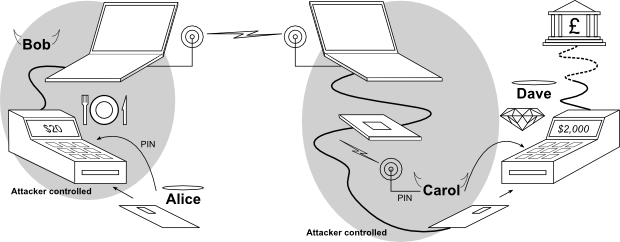
\includegraphics[width=0.5\textwidth]{sc-relay}
\caption{Relay attack depiction in real world scenario}
\end{figure}

\subsection{Countering relay attacks}
An effective countermeasure solution against the relay attack addressed here will be
an implementation that will work within the operating constraints of the existing ECMA and ISO standards. By giving a little change to the software program at the reader or
initiator we are able to in essence provide a solution with a software program or perhaps firmware update.
This wouldn't create changes to any of the existing tags, which have already been manufactured and distributed. Rather changes will remain limited to the readers,
and could produce an an easy-to-implement and affordable solution to our issue. We
don't propose a change to any of the standards, to the communication techniques or
anything to compromise alternate tag type compatibility, but rather a time based two-factor authentication mechanism to detect and counter possible relay attempts.
This remedy has been implemented and tested with Mifare Classic 1K card. We have used a typical NFC tag to emulate our security protocol that asks for a pin if it takes longer than the threshold time used for indicating a possible relay attack.For more security this implementation could allow for any alert mechanism along with pin requirement .
If different tag types were to be used additional research
into timing for those tags should be evaluated. We want this particular solution to be robust
against practical relay attacks and consistent in its warnings and not ask for pin for every genuine transaction as well. To implement this in devices that are Android for instance a
quick code update could create the time based two-factor authentication protocol needed to protect against relay attacks and could be pushed out to the devices as any normal software update would be.
\section{Contactless Payment System}
From new form factors like watches and phones, to new acceptance locations - like vending machines - contactless payment technology is actually fueling innovation in the payments industry. Issuers
and payment brands have introduced a variety of form factors including fobs, mini cards, stickers,
mobile phones and wearables (jewellery, wristwatches and wristbands) - all enabled with contactless payment.
As a result, consumers now view contactless as an established payment method for low value general retail transactions, ticketing and transport, and toll or perhaps parking transactions.
And contactless is actually happening on the mobile in a huge way. Already available in the US, Canada and
Australia, Apple Pay - Apple's mobile payment and digital wallet service has recently launched or will launch in China, Hong Kong, Spain and Singapore. Apple isn't alone. Google, Samsung and Android have implemented contactless payment using Host-Card emulation on devices. Indeed, Samsung is actually taking things even more with
plans to extend service beyond payment to transit passes, coupons and membership cards - an approach also possible on today's multi- application contactless payment cards.NFC technology is emerging as a helpful accessory for consumer transactions. NFC is not a payment technology; it's a set of standards that
enables proximity based communication between consumer electronic devices like mobile phones, tablets, wearable devices or perhaps personal computers. An NFC enabled mobile device is able to communicate with
a POS system that currently accepts contactless payment cards. Contactless payment transactions can
be made using NFC enabled devices that are actually provisioned with a mobile
payment application and are actually processed the same as contact and contactless EMV chip card transactions.
\begin{figure}[h]
\includegraphics[width=0.5\textwidth]{cc}
\caption{Credit Card Payment System}
\end{figure}
\subsection{Devices in Contacless Payments}
Almost any device capable of making payments using radio frequency identification (RFID) technology is actually using contactless payment technology. The device doesn't have to be a smartphone though this is by far the most commonly used device for contactless payments. An antenna and NFC chip embedded into the device lets the customer wave their smartphone over a card reader to create a purchase. Our work here is related specifically to NFC enabled credit cards and preventing relay attacks on them. Apple-pay is secure because of it's two-factor authentication as it asks for passcode or fingerprint before sending information through NFC and uses secure chip to store its confidential data to protect from data theft in this case card details.

Security for contactless payments in credit card does not have the feature of two factor authentication for practical reasons. A user wants to use NFC to pay and entering a pin every time is not efficient. Fraud protection laws all apply, and secure channels and encryption are actually used for sending credit card info and PIN numbers. For several purchases or high priced purchases within a very short period of time, the user is actually asked to manually enter the PIN number to ensure theft hasn't occurred. Typically contactless payments are faster because the PIN number or even a signature is not necessary. It also, nonetheless, can result in the customer to spend much more since paying is very quick and easy.

The very first example of contactless payment came in the form of Speedpass in 1997. Mobil gas stations offered contactless payment devices that clipped onto a key ring. The customer waved the device over a labeled square at the gas pump and paid instantly. Today ExxonMobil still offers this service, and other gas stations are actually incorporating contactless payment technologies into their payment choices.
\subsubsection{Working of NFC Credit Card}
In order to understand the working of our solution it is important to understand the working of a contactless payment system. In the normal functioning of contactless transaction through credit card,The first step is that the reader sends an unpredictable number to the credit card which uses this input along with the Automatic transaction counter(ATC) which is stored in the discretionary data field of the card and uses the inbuilt special NFC chip for credit cards that is made use of to compute a dynamic CVV as well as for encryption purposes.The card then sends the newly generated dynamic CVV along with the ATC in encrypted format to the POS. The POS verifies this CVV with the provided ATC and sends this information to the appropriate bank for approval. The latter part is not important as it is verification by the bank system which  does not involve the security the security of NFC credit cards. The use of dynamic CVV adds greater security to NFC cards as it acts like one time password for the credit cards. So even if a person is able to store the details of the relayed credit card and emulate it, it cannot be successful in using the cards for malicious purposes due to this feature.

\section{Proposed Solution}
\begin{figure}[h]
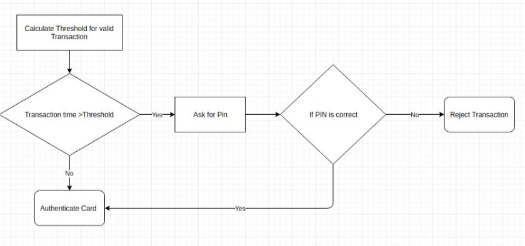
\includegraphics[width=0.5\textwidth,height=0.3\textheight]{Flow}
\caption{Proposed Architecture}
\end{figure}
In the following section we present an approach to detect relay attacks by monitoring the communication delays caused by relay medium used and the processing of the data received at each malicious device and by responding to timing anomalies. The premise for this
work is actually that (a) we are able to see just how long it takes to communicate with a tag and
(b) If the threshold selected to mark the maximum time it takes for a legit transaction then using that threshold it can predict the likelihood of whether or not a relay attack is actually occurring. To be able to be feasible, this solution requires an accurate analysis
of the consistency of timing between different cards. A timing based anomaly detection is only
as accurate as the underlying behavior is actually predictable. Once timing is actually shown to be
consistent we proceed to demonstrate that the implementation of a practical relay attack detection is actually possible at low cost .To be able to collect tag read latency and relay latency data we implemented a relay system. A breakdown of the tag communication steps at a low level can help us with understanding where any timing anomalies occur. We are going to show that the actual time it takes to read a Mifare Classic 1k Card which has certain data bytes and then evaluating delay over the relay system to read the same card. This enables us to distinguish between the actual legit transaction which takes time that is lower than or equal to the selected threshold and a relay attack that takes time that is higher than the selected threshold. Using this  demonstrate that it's preventable and detectable. To avoid delays that are caused by anamolies and not by relay attack we add a pin authentication step to let a legit user use the card. In this way the two-factor authentication is required only when the reader predicts that a relay attack is probably happening.In this case if the user is asked for a pin he/she can continue with the transaction as shown in figure 5. If the attacker is asked for the pin, he/she cannot possibly guess the correct pin and the transaction will fail as shown in figure 6.
\begin{figure}[h]
\includegraphics[width=0.5\textwidth,height=0.2\textheight]{graph}
\caption{Average Time Chart}
\end{figure}
\section{Implementation}
\subsubsection{Emulating relay attacks}
To display the working of a relay attack, we have used PN532 NFC reader along with Raspberry Pi connected to a Linux laptop-(ASUS XJ550) running on Ubuntu operating system.We measure the time for every step in relay attack and use SSH to send the Mifare Classic card data over WiFi to the proxy laptop.We also measure the time required for the same card without the relay apparatus.It has been noted that the time difference in actual transaction and the time taken to relay the information from the malicious reader to the malicious slave device is approximately on an average 500 milliseconds.This helps in deciding the threshold to indicate a relay attack has a difference of 500 milliseconds which is quite huge.
First we measure the time taken to just read the NFC credit card and then we run a shell script which reads the card and then secure copies the primary database file in this case dump.mfd to the connected linux laptop that plays the role of proxy device in this setup. We also noted that the time to just transfer the dump.mfd file was 18 milliseconds on an average. This represents the time to relay information from mole to proxy device . Time difference greater than 5 milliseconds is significant here as the legitimate transaction mostly showed a +3 or -3 variation. Given that the time difference to relay from mole to proxy being high, the time to relay from proxy to POS is just going to add a few more milliseconds which won't make such a great difference in this architecture.  We run the same experiment many times to come to a conclusion that relay attack always took more time than a legit transaction and the time difference was the factor that helped us in detecting a relay attack.Our experiment excludes giving importance to the time difference it took to process the transaction at stack level as it will vary from hardware to hardware. In our case it was around 450 milliseconds on an average. 
\subsubsection{Emulating Time-Based Two Factor Authentication}
We have used PN532 Adafruit NFC Shield and Arduino Uno microcontroller version 3 and Arduino IDE and AdaFruit NFC Library.We  emulated the relay attack detection and pin authentication to prevent possible relay attack.Time taken to read the MiFare Classic card having the same amount of data for each reading was taken as a threshold for indicati ng relay attacks.According to the proposed solution a relay attack will always take more time than this threshold and hence can be detected.To consider any other network failure 
that may cause delay in a legit transaction,we've added a pin authentication feature to authenticate the original user in these situations.As the attacker is not aware of the pin he cannot continue with the transaction even after relaying everything.Arduino was used for simulation of  the pin authentication feature,to do this we added a small delay that represents the relay attack.This delay causes the reader program to ask for a pin to authenticate the user. 
\begin{figure}[h]
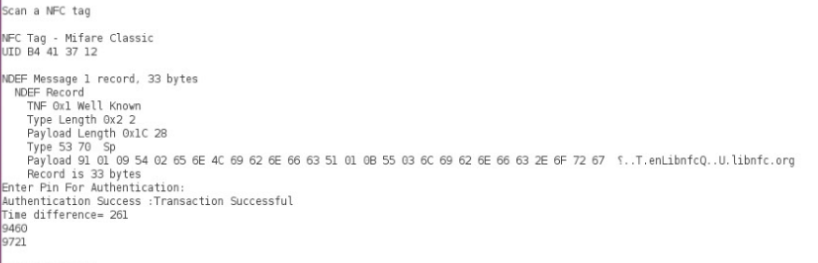
\includegraphics[width=0.5\textwidth,height=0.2\textheight]{spin}
\caption{Pin Authentication for possible relay detection : Success for User}
\end{figure}
\begin{figure}[h]
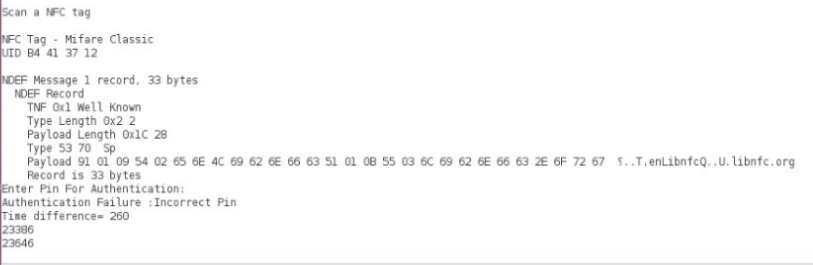
\includegraphics[width=0.5\textwidth,height=0.2\textheight]{fpin}
\caption{Pin Authentication for possible relay detection :Failure for Attacker}
\end{figure}




























% An example of a floating figure using the graphicx package.
% Note that \label must occur AFTER (or within) \caption.
% For figures, \caption should occur after the \includegraphics.
% Note that IEEEtran v1.7 and later has special internal code that
% is designed to preserve the operation of \label within \caption
% even when the captionsoff option is in effect. However, because
% of issues like this, it may be the safest practice to put all your
% \label just after \caption rather than within \caption{}.
%
% Reminder: the "draftcls" or "draftclsnofoot", not "draft", class
% option should be used if it is desired that the figures are to be
% displayed while in draft mode.
%
%\begin{figure}[!t]
%\centering
%\includegraphics[width=2.5in]{myfigure}
% where an .eps filename suffix will be assumed under latex, 
% and a .pdf suffix will be assumed for pdflatex; or what has been declared
% via \DeclareGraphicsExtensions.
%\caption{Simulation results for the network.}
%\label{fig_sim}
%\end{figure}

% Note that the IEEE typically puts floats only at the top, even when this
% results in a large percentage of a column being occupied by floats.


% An example of a double column floating figure using two subfigures.
% (The subfig.sty package must be loaded for this to work.)
% The subfigure \label commands are set within each subfloat command,
% and the \label for the overall figure must come after \caption.
% \hfil is used as a separator to get equal spacing.
% Watch out that the combined width of all the subfigures on a 
% line do not exceed the text width or a line break will occur.
%
%\begin{figure*}[!t]
%\centering
%\subfloat[Case I]{\includegraphics[width=2.5in]{box}%
%\label{fig_first_case}}
%\hfil
%\subfloat[Case II]{\includegraphics[width=2.5in]{box}%
%\label{fig_second_case}}
%\caption{Simulation results for the network.}
%\label{fig_sim}
%\end{figure*}
%
% Note that often IEEE papers with subfigures do not employ subfigure
% captions (using the optional argument to \subfloat[]), but instead will
% reference/describe all of them (a), (b), etc., within the main caption.
% Be aware that for subfig.sty to generate the (a), (b), etc., subfigure
% labels, the optional argument to \subfloat must be present. If a
% subcaption is not desired, just leave its contents blank,
% e.g., \subfloat[].


% An example of a floating table. Note that, for IEEE style tables, the
% \caption command should come BEFORE the table and, given that table
% captions serve much like titles, are usually capitalized except for words
% such as a, an, and, as, at, but, by, for, in, nor, of, on, or, the, to
% and up, which are usually not capitalized unless they are the first or
% last word of the caption. Table text will default to \footnotesize as
% the IEEE normally uses this smaller font for tables.
% The \label must come after \caption as always.
%
%\begin{table}[!t]
%% increase table row spacing, adjust to taste
%\renewcommand{\arraystretch}{1.3}
% if using array.sty, it might be a good idea to tweak the value of
% \extrarowheight as needed to properly center the text within the cells
%\caption{An Example of a Table}
%\label{table_example}
%\centering
%% Some packages, such as MDW tools, offer better commands for making tables
%% than the plain LaTeX2e tabular which is used here.
%\begin{tabular}{|c||c|}
%\hline
%One & Two\\
%\hline
%Three & Four\\
%\hline
%\end{tabular}
%\end{table}


% Note that the IEEE does not put floats in the very first column
% - or typically anywhere on the first page for that matter. Also,
% in-text middle ("here") positioning is typically not used, but it
% is allowed and encouraged for Computer Society conferences (but
% not Computer Society journals). Most IEEE journals/conferences use
% top floats exclusively. 
% Note that, LaTeX2e, unlike IEEE journals/conferences, places
% footnotes above bottom floats. This can be corrected via the
% \fnbelowfloat command of the stfloats package.
\section{Limitation}
This solution is time based which in turn depends on the hardware used in the transaction. Readers have to be faster and process transactions at higher speeds. If a attacker is overclocking its readers to increase their speed and manages to run the relay attack faster than the payment terminal processes a valid transaction, then that relay attack cannot be detected. The only solution here will be to overclock the payment terminals as well which would increase the energy consumption and and decrease the hardware lifetime. 
 



\section{Conclusion}
NFC is now a rapidly growing technology. It surrounds us today and will
continue to in the near future. We've all seen the effects of malicious parties taking
benefit of security vulnerabilities in technology fields, and NFC is actually no exception to this. The rapid expansion of the technology and lack of solutions to the security
vulnerabilities are a concern. Relay attacks are a present and real very threat to this
technology, both diffcult to detect and also to stop.
We show in this work that by timing the communication of NFC tags a section at a time during data transmissions we are able to detect relay attacks successfully. The accurate
timing at the proper level is crucial in this particular endeavor. After detection, many different
actions may be taken. One particular action might be a system that first issues warnings,
then completely stops communication.
By taking a look at the time needed for a data read on a tag we are able to preserve the
existing technologies by sticking with the ISO specifications and enhance security at the same time. This won't result in significant changes to the protocols or perhaps the existing
devices on the market today. It would just need a software update at the reader side, i.e. POS. In probably the worst case this solution would ask for a pin from an end user for most of the transactions as it probably detects the chance of a relay attack, and also can allow all current NFC
devices to work under the established protocols and simply alert them of potential malicious activity. Applying a solution such as this to it within the current
ISO specifications without causing expense or changes significantly is important and this particular solution is that criteria.
This technology benefits many industries as well as allows for applications in fields which could be very advantageous. We expect that the solutions presented
here will add both a level of security as well as value to NFC technology.The effectiveness and ease of the attack means that
ticketing, payment (mobile wallets and credit card) and
access control application need to be hardened against relay attacks. Currently, virtually no deployed products
implement relay resistant mechanisms, with the exception
of NXP's new Mifare Plus smart card and that has
up to now only seen limited deployment and it's unknown
just how many systems that do use Mifare Plus actually take advantage of this particular security service. There are
a number of countermeasures which are considered
effective against relay attacks, and mobile platforms
have much possibilities when compared to conventional
smart cards





% conference papers do not normally have an appendix


% use section* for acknowledgment
\section*{Acknowledgment}


We would like to thank our Professor Parth Pathak for guiding us and encouraging us to learn about NFC and motivated us to find a way to improve the security of NFC. 





% trigger a \newpage just before the given reference
% number - used to balance the columns on the last page
% adjust value as needed - may need to be readjusted if
% the document is modified later
%\IEEEtriggeratref{8}
% The "triggered" command can be changed if desired:
%\IEEEtriggercmd{\enlargethispage{-5in}}

% references section
% can use a bibliography generated by BibTeX as a .bbl file
% BibTeX documentation can be easily obtained at:
% http://mirror.ctan.org/biblio/bibtex/contrib/doc/
% The IEEEtran BibTeX style support page is at:
% http://www.michaelshell.org/tex/ieeetran/bibtex/
%\bibliographystyle{IEEEtran}
% argument is your BibTeX string definitions and bibliography database(s)
%\bibliography{IEEEabrv,../bib/paper}
%
% <OR> manually copy in the resultant .bbl file
% set second argument of \begin to the number of references
% (used to reserve space for the reference number labels box)
\begin{thebibliography}{1}

\bibitem{IEEEhowto:kopka}
Prevention of Relay Attack Using NFC \emph{Deepa S Pillai1
, S.Sathyalakshmi},\hskip 1em plus
0.5em minus 0.4em\relax PG Scholar, Department of  Computer Science \& Engineering Hindustan University, Padur, Chennai, India
\bibitem{IEEEhowto:kopka}
Practical Relay Attack on Contactless Transactions
by Using NFC Mobile Phones \emph\\{Lishoy Francis, Gerhard Hancke, Keith Mayes, Konstantinos Markantonakis},\hskip 1em plus
0.5em minus 0.4em\relax Information Security Group, Smart Card Centre
Royal Holloway University of London
Egham Hill, TW20 0EX, Surrey, United Kingdom
\bibitem{IEEEhowto:kopka}
Practical Experiences on NFC Relay Attacks
with Android: Virtual Pickpocketing Revisited \emph\\{anonymous}\hskip 1em plus
0.5em minus 0.4em\relax 
\bibitem{IEEEhowto:kopka}
Security in Near Field Communication (NFC) –
Strengths and Weaknesses. In: Proceedings of the Workshop on RFID Security
and Privacy. (2006) 1–11
 \emph\\{ Haselsteiner, E., Breitfuß, K}\hskip 1em plus
0.5em minus 0.4em\relax 
\bibitem{IEEEhowto:kopka}
Nfc attacks analysis and survey.In Innova-
tive Mobile and Internet Services in Ubiquitous Computing (IMIS)
 \emph\\{ C. Chen, I. Lin, and C. Yang.}\hskip 1em plus
0.5em minus 0.4em\relax
\bibitem{IEEEhowto:kopka}
A Relay Prevention Technique For Near Field
Communication
 \emph\\{ ERIC S. WILCOX}\hskip 1em plus
0.5em minus 0.4em\relax
\bibitem{IEEEhowto:kopka}
Relay attacks of NFC smart cards-Xiqing Chu

 \emph\\{ }\hskip 1em plus
0.5em minus 0.4em\relax
\bibitem{IEEEhowto:kopka}
Conditional privacy preserving security protocol for NFC applications
 \emph\\{ 
Eun.H, Lee.H, Son.J, Kim.S, and Oh.H}\hskip 1em plus
0.5em minus 0.4em\relax
\bibitem{IEEEhowto:kopka} 
Access Without Permission: A Practical RFID Relay Attack
 \emph\\{ Roman Silberschneider, Thomas Korak, and Michael Hutter}\hskip 1em plus
0.5em minus 0.4em\relax 
\bibitem{IEEEhowto:kopka} 
Relaying EMV Contactless Transactions using
Off-The-Shelf Android Devices
 \emph\\{J. van den Breekel}\hskip 1em plus
0.5em minus 0.4em\relax 
\bibitem{IEEEhowto:kopka} 
Relay Cost Bounding for Contactless EMV Payments
 \emph\\{T. Chothia, F. D. Garcia, J. de Ruiter, J. van den Breekel, M. Thompson}\hskip 1em plus
0.5em minus 0.4em\relax 
\bibitem{IEEEhowto:kopka} 
Picking Virtual Pockets using Relay Attacks on
Contactless Smartcard
 \emph\\{Z. Kfir, A. Wool}\hskip 1em plus
0.5em minus 0.4em\relax 
\end{thebibliography}




% that's all folks
\end{document}


